\documentclass[a4paper,12pt]{extarticle}
% !TEX encoding = IBM866
\usepackage[T2A]{fontenc}
\usepackage{listings}
\usepackage[dvipsnames]{xcolor}
\usepackage{algorithm2e}
\usepackage{array}
\usepackage{moreverb}
\usepackage{multirow}

\usepackage[russian]{babel}
\usepackage{amsthm,amsmath,amsfonts,amssymb}
\usepackage[final]{graphicx}
\usepackage{float}
\usepackage{geometry}
\geometry
{
a4paper,
total={210mm,297mm},
left=20mm,
right=20mm,
top=25mm,
bottom=20mm,
}

\usepackage{tikz}
\usepackage{pgfplots}
\usepackage[final]{showkeys}

\usepackage{caption}
\DeclareCaptionLabelSeparator{dot}{. }
\captionsetup{labelsep=dot}

\usepackage{hyperref}
\usepackage{lastpage}
\usepackage{fancyhdr}



\begin{document}


    \begin{titlepage}

        \begin{center}
            \centerline{\Large\rm Министерство науки и высшего образования}
            \centerline{\Large\rm Федеральное государственное бюджетное образовательное}
            \centerline{\Large\rm учреждение высшего образования}
            \centerline{\Large\rm <<Московский государственный технический университет}
            \centerline{\Large\rm имени~Н.~Э.~Баумана}
            \centerline{\Large\rm (национальный исследовательский университет)>>}
            \centerline{\Large\rm (МГТУ~им.~Н.~Э.~Баумана)}
            \hrulefill
        \end{center}

        \begin{figure}[h!]
            \centering
            
\includegraphics[height=0.4\linewidth]{picture0}
        \end{figure}

        \begin{center}
            \centerline{\Large\rm Факультет <<Фундаментальные науки>>}
            \centerline{\Large\rm Кафедра ФН1 <<Высшая математика>>}
            \centerline{\Large\rm Дисциплина <<Методы вычислений>>}
        \end{center}

        \begin{center}
            \textsc{\textbf{\Huge Отчет}}\\
            \textsc{\textbf{\large по лабораторной работе №3}}\\
        \end{center}

        \vspace{3em}

        {
        \large
        \hbox to 17cm {Преподаватель \hspace{45pt} \hrulefill \hspace{60pt} Коновалов~Я.~Ю.}
        \vspace{-7pt}
        \hbox{{\small\it \hspace{178pt} подпись, инициалы}}
        \hbox{}
        \hbox to 17cm {Студенты группы ФН1--51Б \hrulefill \hspace{1pt} Терновой~Е.~А. и Гончаров~М.~В.}
        \vspace{-7pt}
        \hbox{{\small\it \hspace{178pt} подпись, инициалы}}
        }


        \vspace{\fill}

        \begin{center}
            \large    Москва \\2020
        \end{center}

    \end{titlepage}

    \setcounter{page}{2}
    \tableofcontents
    \vspace{\baselineskip}

    \newpage


    \section{Задание}
    Используя численные методы(Деление отрезка пополам, секущие, касательные), найти решение уравнений $f(x) = 0$ на заданном отрезке. Обосновать единственность полученного решения на этом отрезке для следующих функций:

    \begin{enumerate}
        \item $f_1(x) = x(x-3)(x-4)$
        \item $f_2(x) = e^x + \cos x$
        \item $f_3(x) = x^{10} - 2x^9 + 3x^8 - x^7 + 5x^6 + x^5 - x^4 - x^3 + x^2 - x$
    \end{enumerate}

    \begin{figure}[h!]
        \centering
        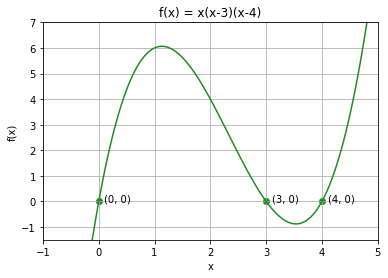
\includegraphics[height=0.5\linewidth]{1.png}
        \caption{Полином низкого порядка}
        \label{fig:res1}
    \end{figure}

    \begin{figure}[h!]
        \centering
        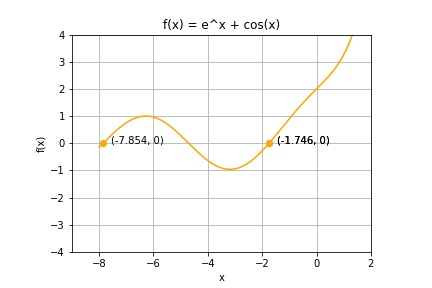
\includegraphics[height=0.5\linewidth]{2.jpg}
        \caption{Трансцендентная функция}
        \label{fig:res2}

    \end{figure}

    \begin{figure}[h!]
        \centering
        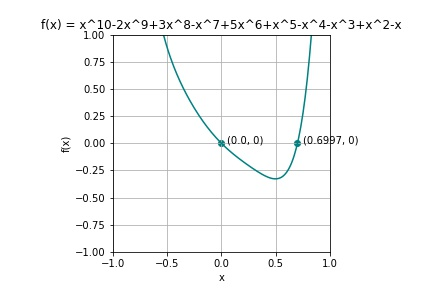
\includegraphics[height=0.5\linewidth]{3.jpg}
        \caption{Полином высокого порядка}
        \label{fig:res3}
    \end{figure}



    \newpage


    \noindent
    В работе указать аналитические методы приближения, кол--во итераций для каждого из методов, при которых достигается точность $\varepsilon = 10^{-5}$, время вычисления корня.
    \section{Аналитическое решение и локализация корней}

    \subsection{Теорема}
    Если функция $f(x)$ непрерывна на отрезке $[a; b]$ и на концах отрезка принимает ненулевые значения разных знаков т.е. $f(a)\cdot f(b) < 0$, то на данном интервале найдется по
    крайней мере одна точка $\xi$ в которой $f(\xi) = 0$.

    \subsection{Полином низкого порядка}

    \[
        f(x) = x(x-3)(x-4) = x^3 - 7x^2 + 12x
    \]

    \begin{figure}[h!]
        \centering
        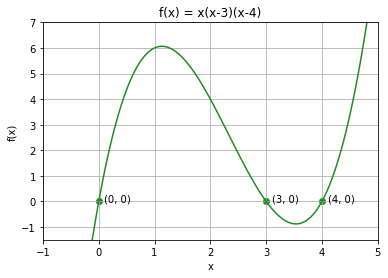
\includegraphics[height=0.5\linewidth]{1.png}
        \caption{$f(x) = x^3 - 7x^2 + 12x$}
    \end{figure}

    Исходя из графика, выберем интервал $x \in [-2, 1]$

    \[
        f(-2)f(1) < 0
    \]

    Исходя их теоремы, можно сделать вывод, что интервал $[-2, 1]$ содержит хотя бы одно решение.
    График является подтвержением того, что на данном интервале действительно есть ровно одно решение.

    \newpage

    \subsection{Трансцендентная функция}

    \[
        f(x) = e^x + \cos x
    \]

    \begin{figure}[h!]
        \centering
        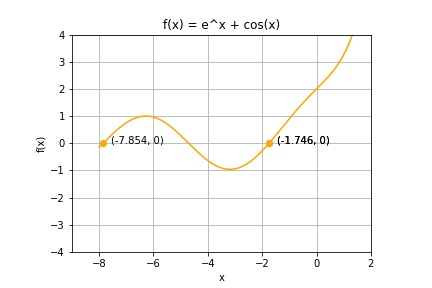
\includegraphics[height=0.6\linewidth]{2.jpg}
        \caption{$f(x) = e^x + \cos x$}
    \end{figure}

    Исходя из графика, выберем интервал $x \in [-2, 0]$

    \[
        f(-2)f(0) < 0
    \]

    Исходя их теоремы, можно сделать вывод, что интервал $[-2, 0]$ содержит хотя бы одно решение.
    График является подтвержением того, что на данном интервале действительно есть ровно одно решение.

    \newpage

    \subsection{Полином высокого порядка}

    \[
        f(x) = x^{10} - 2x^9 + 3x^8 - x^7 + 5x^6 + x^5 - x^4 - x^3 + x^2 - x
    \]

    \begin{figure}[h!]
        \centering
        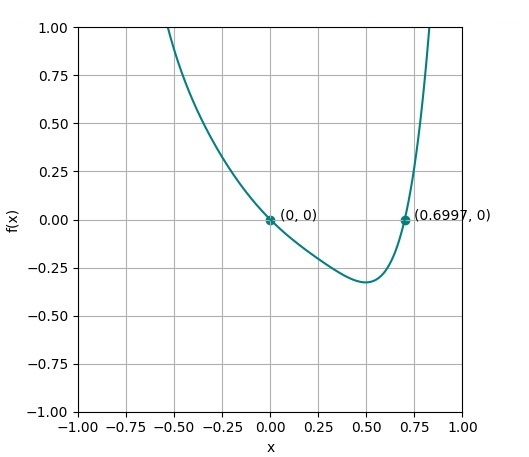
\includegraphics[height=0.6\linewidth]{plot3_3}
        \caption{$f(x) = x^{10} - 2x^9 + 3x^8 - x^7 + 5x^6 + x^5 - x^4 - x^3 + x^2 - x$}
    \end{figure}

    Исходя из графика, выберем интервал $x \in [-1, 0.5]$

    \[
        f(-1)f(0.5) < 0
    \]

    Исходя их теоремы, можно сделать вывод, что интервал $[-1, 0.5]$ содержит хотя бы одно решение.
    График является подтвержением того, что на данном интервале действительно есть ровно одно решение.

    \newpage


    \section{Код программы}

    \subsection{Метод дихотомии отрезка}
    \listinginput[1]{1}{DichotomyMethod.java}

    \newpage

    \subsection{Метод секущих}
    \listinginput[1]{1}{SecantMethod.java}

    \newpage

    \subsection{Метод касательных}
    \listinginput[1]{1}{NewtonMethod.java}

    \newpage


    \section{Результаты работы программы}

    \subsection{$f_1(x) = x(x-3)(x-4)$}

    \begin{center}
        \begin{tabular}{ |c|c|c|c|c| }
            \hline
            Метод       & кол--во итераций & Числ. знач.           & $\Delta t$, с       \\
            \hline
            Дихотомия   & 35               & $-2.91\cdot 10^{-11}$ & $1.02\cdot 10^{-5}$ \\
            \hline
            Секущие     & 6                & $6.76\cdot 10^{-34}$  & $1.26\cdot 10^{-5}$ \\
            \hline
            Касательные & 7                & $-8.99\cdot 10^{-29}$ & $7.47\cdot 10^{-5}$ \\
            \hline
        \end{tabular}
    \end{center}

    \subsection{$f_2(x) = e^x + \cos x$}

    \begin{center}
        \begin{tabular}{ |c|c|c|c|c| }
            \hline
            Метод       & кол--во итераций & Числ. знач.           & $\Delta t$, с       \\
            \hline
            Дихотомия   & 36               & $-1.746139530383516$  & $2.39\cdot 10^{-5}$ \\
            \hline
            Секущие     & 3                & $-1.7461395304080125$ & $3.83\cdot 10^{-5}$ \\
            \hline
            Касательные & 10               & $-1.746139530419238$  & $2.2\cdot 10^{-5}$  \\
            \hline
        \end{tabular}
    \end{center}

    \subsection{$f_3(x) = x^{10} - 2x^9 + 3x^8 - x^7 + 5x^6 + x^5 - x^4 - x^3 + x^2 - x$}

    \begin{center}
        \begin{tabular}{ |c|c|c|c|c| }
            \hline
            Метод     & кол--во итераций & Числ. знач.                        & $\Delta t$, с       \\
            \hline
            Дихотомия & 34               & $2.91\cdot 10^{-11}$ & $4.55\cdot 10^{-5}$ \\
            \hline
            Секущие & 8                & $3.67\cdot 10^{-39}$ & $6.31\cdot 10^{-5}$ \\
            \hline
            Касательные & 9                & $-8.29\cdot 10^{-23}$ & $4.92\cdot 10^{-5}$ \\
            \hline
        \end{tabular}
    \end{center}

    \centering{\LaTeX}

\end{document}